\chapter{Fundamentação teórica}

Este capítulo aborda os conceitos teóricos necessários para a compreensão do presente trabalho.

\section{Aprendizado de Máquina}

O aprendizado de máquina é um subcampo da inteligência artificial que tem por objetivo o desenvolvimento de algoritmos capazes de aprender e tomar decisões a partir de um conjunto de dados, sem que seja necessária a programação explícita para essas tarefas específicas \cite{mlDietterich}. Fundamentalmente, esses sistemas buscam aprender padrões em coleções de dados para, a partir da generalização desse conhecimento, realizar inferências sobre novas informações. Esse processo de aprendizado utiliza modelos matemáticos, principalmente estatísticos, que capturam relações complexas entre variáveis de entrada e saída através do ajuste de parâmetros internos, permitindo que a aplicação melhore seu desempenho conforme é exposta a mais dados \cite{mlSarker}. Em geral, as técnicas de \textit{machine learning} são categorizadas em três paradigmas principais: aprendizagem supervisionada, não supervisionada e por reforço.

O aprendizado supervisionado caracteriza-se pela utilização de conjuntos de dados rotulados, onde tanto as entradas quanto as saídas desejadas são conhecidas durante o treinamento. Nesse paradigma, o algoritmo aprende através de exemplos, de forma a possibilitar tarefas como classificação — a atribuição de classes discretas aos dados — e regressão — a predição de valores contínuos. Algoritmos clássicos dessa categoria incluem máquinas de vetores de suporte, redes neurais artificiais e métodos \textit{ensemble} \cite{mlSarker}. O aprendizado não-supervisionado, por sua vez, opera sobre dados não rotulados, sem o conhecimento das saídas desejadas, e busca compreender a organização natural de um dado conjunto a partir da identificação de padrões intrínsecos. Essa abordagem engloba técnicas como agrupamento (\textit{clustering}) e detecção de anomalias \cite{mlSarker}. Ainda, diferentes estratégias de aprendizado podem ser incorporadas, como algoritmos semi-supervisionados, utilizados quando um \textit{dataset} tem poucos dados classificados, de forma a aproveitar a estrutura implícita do conjunto não categorizado para melhorar o desempenho do modelo \cite{mlSarker}.

Adicionalmente, o aprendizado por reforço representa um paradigma distinto onde um modelo aprende através de interações com um ambiente, sendo recompensado ou penalizado com base em suas ações, de forma que gradualmente desenvolva estratégias ótimas. Essa abordagem é especialmente útil em áreas como teoria de jogos ou inteligência de enxame \cite{mlSarker}.

Embora os conceitos fundamentais de aprendizado de máquina tenham sido estabelecidos há quase um século, com contribuições embrionárias nas décadas de 1950 e 1960 \cite{mlDietterich}, essa área de estudo tem recebido grande destaque nas últimas décadas. Esse ressurgimento deve-se principalmente ao aumento exponencial da capacidade computacional e a disponibilidade massiva de dados digitais. Também, a evolução do \textit{hardware}, particularmente o advento de unidades de processamento gráfico de alto desempenho, possibilitou o treinamento de modelos complexos, antes computacionalmente intratáveis, transformando o aprendizado de máquina em uma tecnologia fundamental para aplicações modernas em diversas áreas \cite{mlSarker}.

\section{Redes Neurais Profundas}

Redes neurais profundas, comumente utilizadas no paradigma de aprendizado supervisionado, são uma especialização de redes neurais artificiais. Diferentemente das técnicas tradicionais de \textit{machine learning}, que requerem a engenharia manual de características, são capazes de autonomamente aprender representações complexas de um determinado conjunto de dados brutos. Isso é possível por sua estrutura multicamada, que permite a extração progressiva de características de baixo nível -- em uma imagem, por exemplo, bordas e linhas -- até padrões de alto nível -- no mesmo exemplo, objetos e faces \cite{efficientdeep}.

A unidade mais básica de uma rede neural artificial é um neurônio artificial (que será referido aqui apenas como neurônio ou nó).

\begin{figure}[H]
	\caption{\label{fig:neuron}Representação de um Neurônio Artificial}
    \begin{center}
    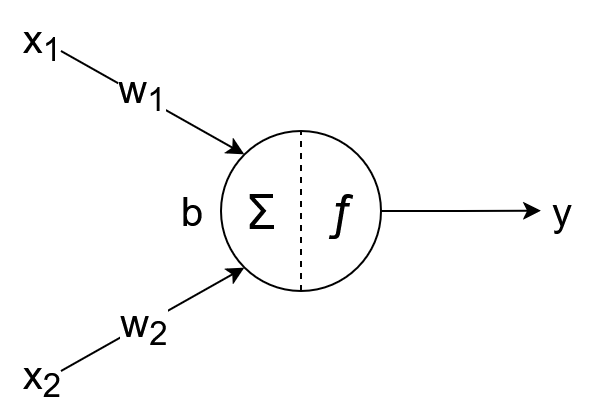
\includegraphics[width=0.7\linewidth]{images/neuron.png}
	\end{center}
	\fonte{o autor}
\end{figure}

No exemplo representado na figura \ref{fig:neuron}, um neurônio recebe dados de entrada, $x_1$ e $x_2$, e produz uma saída $y$. Para isso, cada entrada é multiplicada por seu respectivo peso, $w_1$ e $w_2$, e somada junto a um termo de viés $b$ -- assim, a equação resultante é igual a $\sum = x_1 w_1 + x_2 w_2 + b$. Finalmente, aplica-se uma função de ativação $f$ sobre a soma para converter esse valor em um intervalo desejado -- a tangente hiperbólica produziria um número dentro do intervalo $(-1, 1)$, enquanto a sigmoid produziria um intervalo entre $(0, 1)$, por exemplo -- resultando na saída $y$ \cite{deeplearningbook}. Em outras palavras, os pesos indicam a importância, ou força, da conexão entre a entrada e o neurônio; o viés atua como um limiar de ativação que independe das entradas; e a função de ativação transforma uma entrada linear em uma saída não linear, o que permite um mapeamento complexo entre entradas e saídas. 

Uma rede neural artificial é formada pela interligação de neurônios, assim, uma camada da rede é denominada a partir de um grupo de nós interligados, que processam dados de uma maneira específica. Combinando uma camada de entrada, camadas intermediárias e uma camada de saída, obtém-se uma rede neural profunda, ilustrada na figura \ref{fig:dnn}. Dessa forma, cada camada recebe entradas ponderadas a partir das camadas anteriores, aplicam uma função de ativação e propagam o resultado para as camadas subsequentes \cite{deeplearningbook}. Diferentes configurações destas, como a variação das conexões entre neurônios ou o emprego de funções de ativação distintas, tem por efeito especializações, ou habilidades de aprendizado específicas, assim, a utilização de múltiplas camadas permite a assimilação de representações hierárquicas complexas. \cite{reviewdeep}.

\begin{figure}[H]
	\caption{\label{fig:dnn}Representação de um Neurônio Artificial}
    \begin{center}
    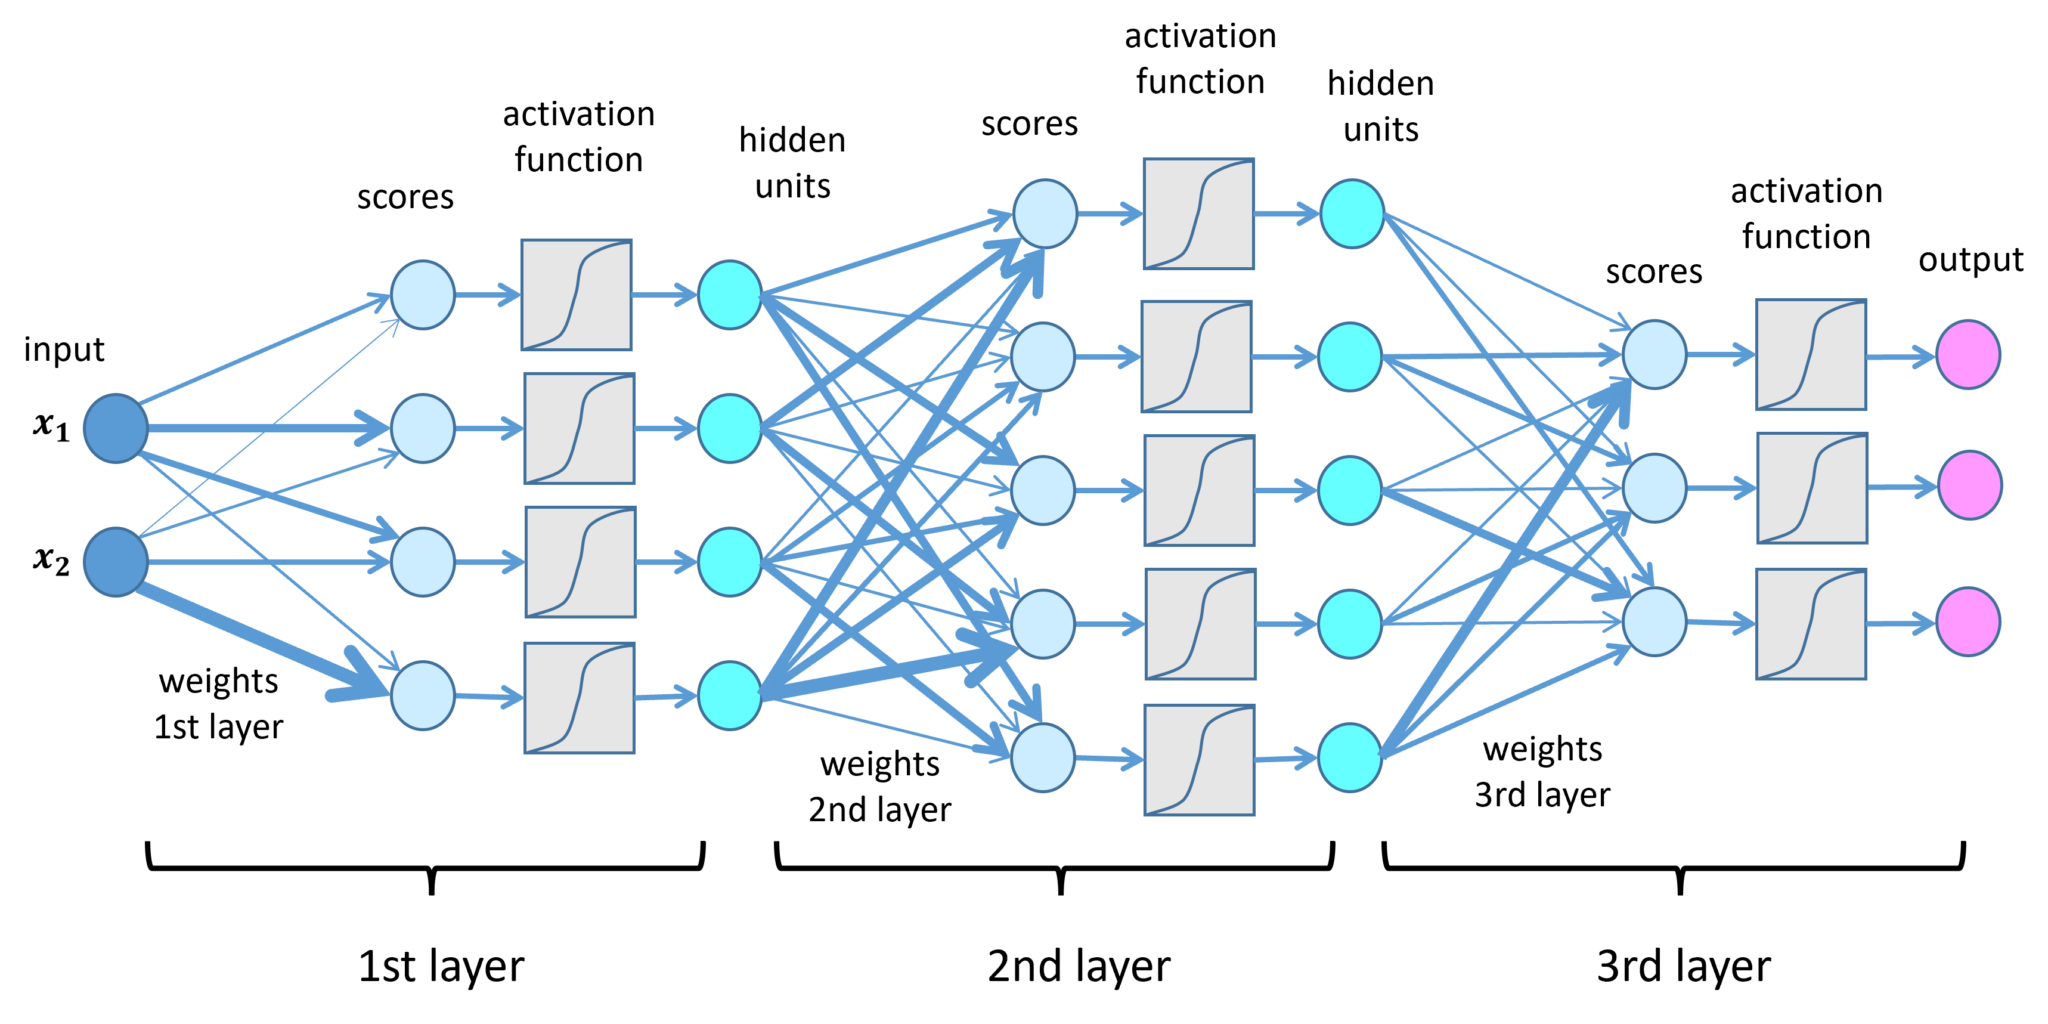
\includegraphics[width=1\linewidth]{images/dnn.png}
	\end{center}
	\fonte{\url{https://lamarr-institute.org/blog/deep-neural-networks/}. Acesso em: 25 junho 2025}
\end{figure}


O processo de aprendizado da rede é denominado treinamento e consiste na estimação e ajuste dos parâmetros através de um algoritmo de retropropagação. Seu objetivo é calcular o gradiente de uma função que mede o erro entre o valor de saída computado e o esperado, além de ajustar os pesos e vieses dos neurônios na direção oposta ao gradiente, para minimizar o erro. Esse processo é executado em cada camada, propagando o erro desde a camada de saída até a de entrada, de forma iterativa, por múltiplas épocas, até que a rede converja para uma solução otimizada \cite{deeplearningbook}, como ilustrado na figura \ref{fig:gradientdescent}, em que o eixo $y$ representa valores de erro e o eixo $x$ valores de peso.

\begin{figure}[H]
	\caption{\label{fig:gradientdescent}Visualização do Gradiente Descendente}
    \begin{center}
    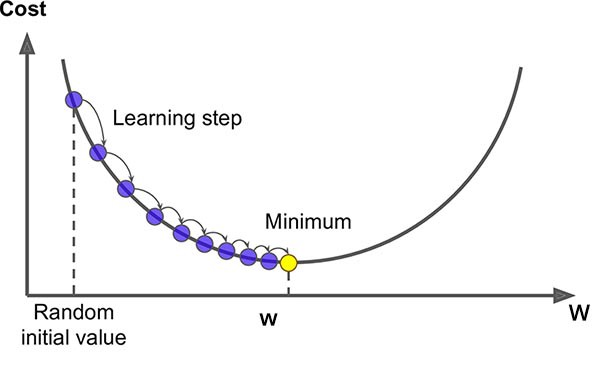
\includegraphics[width=1\linewidth]{images/gradientdescent.jpg}
	\end{center}
	\fonte{\url{https://mlpills.dev/machine-learning/gradient-descent/}. Acesso em: 25 junho 2025}
\end{figure}


\subsection{Redes Neurais Convolucionais}

Redes neurais convolucionais são tipos de redes neurais profundas especialmente úteis na área de visão computacional, especializadas na computação de dados estruturados em topologia de malha, representados matricialmente. O que propicia essa propriedade é o emprego de operações de convolução em pelo menos um módulo da rede, o que consiste em uma mudança no processamento de entrada dos neurônios: ao invés da simples soma ponderada pelos pesos, um cálculo é efetuado a partir da aplicação de um filtro sobre um \textit{input} \cite{deeplearningbook}. Dessa forma, a estrutura de um modelo básico combina camadas convolucionais com camadas de subamostragem, todas esparsamente conectadas \cite{reviewdeep}.

Convolução é uma operação matemática sobre duas funções para a criação de uma terceira, que representa, em termos simplórios, a sobreposição delas. No contexto de redes convolucionais, consiste na multiplicação de duas matrizes seguida de uma soma \cite{origindl}, como demonstrado na figura \ref{fig:convolution}.

\begin{figure}[H]
	\caption{\label{fig:convolution}Visualização de uma Operação de Convolução}
    \begin{center}
    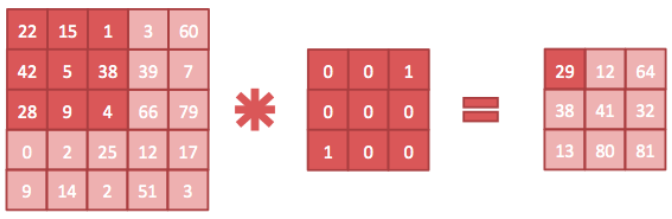
\includegraphics[width=0.75\linewidth]{images/convolution.png}
	\end{center}
	\fonte{\cite{origindl}}
\end{figure}


Um filtro -- ou \textit{kernel}, matrizes de parâmetros aprendíveis -- desliza sobre os dados de entrada, a um passo definido, computando o produto escalar entre seus pesos e os valores correspondentes na região coberta, de forma a criar um mapa de características que representa a presença de padrões específicos detectados pelo filtro \cite{deeplearningbook}. Dessa forma, certas configurações, como o tamanho e os pesos do \textit{kernel}, ou o número de passos de deslizamento, controlam a resolução espacial e a capacidade de modelar relações de vizinhança, como figurativamente representado na figura \ref{fig:nono}, em que a escolha de um filtro inicial para a detecção de bordas permite o treinamento da rede para a distinção entre gatos magros e gordos.

\begin{figure}[H]
	\caption{\label{fig:nono}Representação da Classificação de uma Imagem por uma Rede Convolucional}
    \begin{center}
    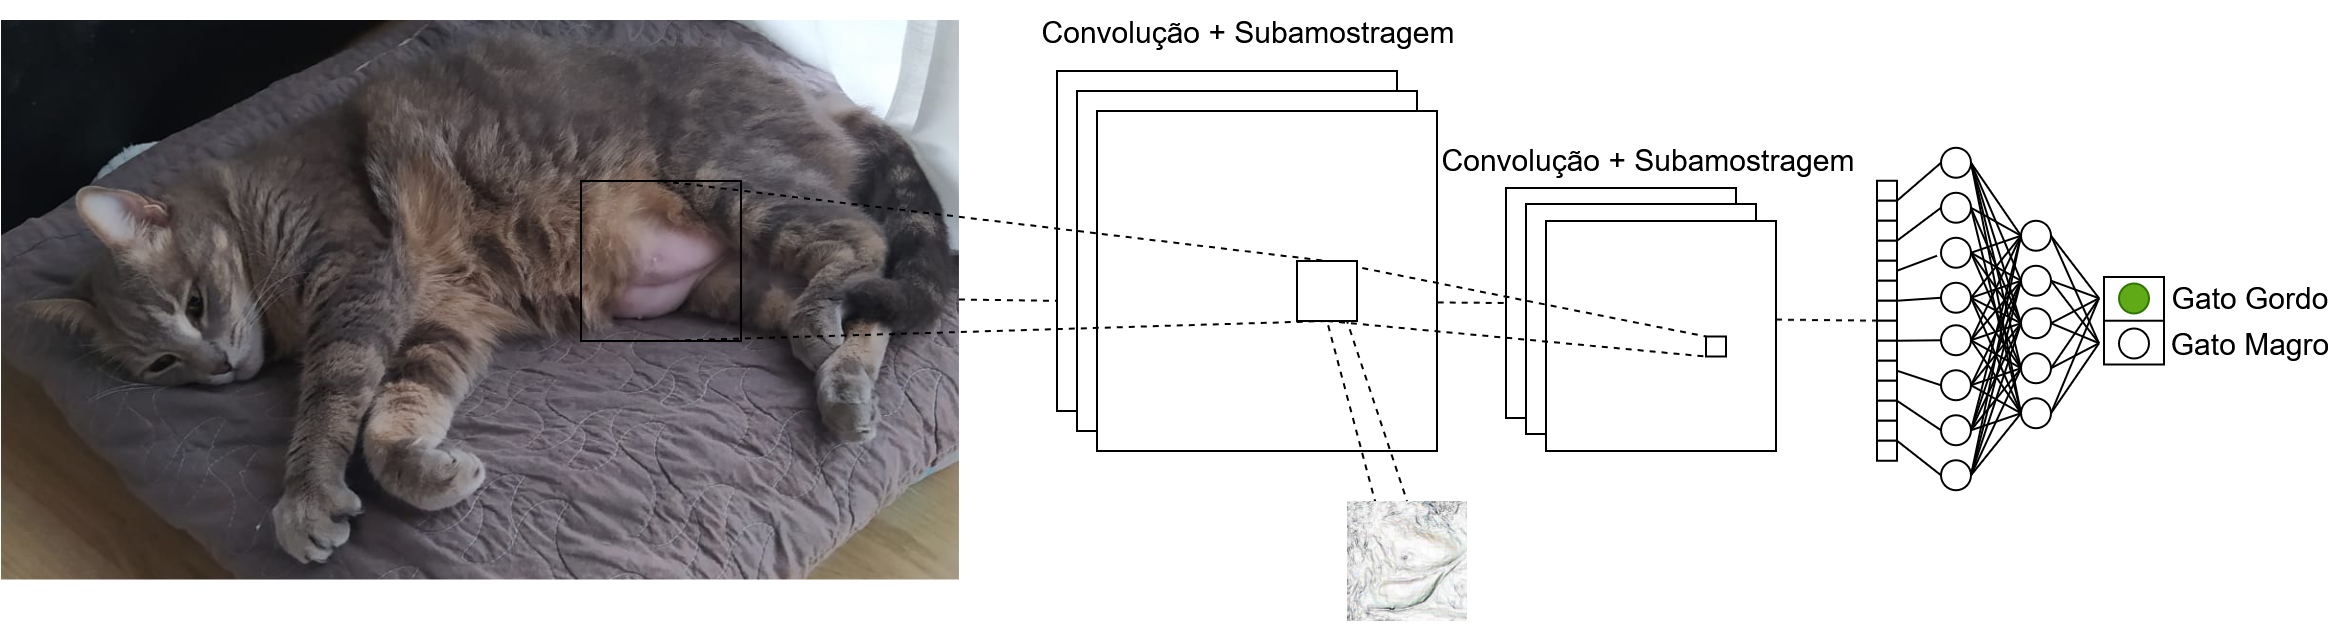
\includegraphics[width=1\linewidth]{images/nono.png}
	\end{center}
	\fonte{o autor}
\end{figure}

Outro importante aspecto das redes convolucionais são as camadas de subamostragem, que reduzem a dimensão espacial dos dados de entrada ao passo em que preservam suas características mais relevantes, processo conhecido como \textit{pooling}. Atingem isso com a obtenção de apenas uma amostra para cada região analisada, para isso, empregam estratégias como \textit{max-pooling} (extração do maior valor de entrada) e \textit{average-pooling} (extração da média dos valores de entrada). A combinação de camadas convolucionais com camadas de subamostragem conferem às essas redes três propriedades fundamentais: a invariância à pequenas transformações, distorções e translações da entrada, que permite que características sejam detectadas independentemente de sua localização; a capacidade de extrair hierarquias espaciais através da redução progressiva de dimensionalidade; e a redução do custo computacional das camadas subsequentes \cite{origindl}.

Dessa forma, a extração de \textit{features} acontece conforme a entrada percorre a rede. Utilizando como exemplo uma imagem para a entrada, as camadas iniciais capturam informações de baixo nível, como bordas, cantos e texturas. Em camadas intermediárias, essas informações passam a compor padrões semânticos locais, como delimitações de objetos, até que, em camadas mais profundas, transformam-se em caracterizações globais de alto nível, como formas completas. Isso permite que as camadas finais possam prever, ou extrair, representações complexas e abstratas \cite{reviewdeep}, como o exemplo utilizado anteriormente -- a classificação entre gatos gordos e magros.

\subsubsection{Reconhecimento Óptico de Caracteres (OCR)}

O reconhecimento óptico de caracteres (OCR), no contexto de computação, descreve um tipo de software que tem por objetivo a conversão de texto, seja impresso ou em imagem, a um formato digital que possa ser processável por máquina \cite{ocr}. É um problema que pode ser tratado utilizando técnicas de segmentação da visão computacional clássica junto a heurísticas, no entanto, as abordagens que utilizam o aprendizado de máquina -- em especial, redes convolucionais -- têm se mostrado mais eficientes e precisas.

De acordo com \citeauthor*{ocr} \cite*{ocr}, um processo de reconhecimento de caracteres moderno tipicamente passa pelo seguinte \textit{pipeline}:

\begin{enumerate}
	\item Aquisição da imagem: obtém-se a imagem com o texto a partir de uma fonte externa, como \textit{scanner} ou câmera;
	\item Pré-processamento: aplicam-se técnicas como remoção de ruído, operações morfológicas e limiarização para melhorar a qualidade da imagem;
	\item Segmentação de caracteres: separam-se os caracteres através da análise de componentes conectados, perfis de projeção ou métodos avançados para tratar textos sobrepostos ou fragmentados;
	\item Extração de \textit{features} e classificação de caracteres: com os caracteres separados, utiliza-se uma rede convolucional para a extração e classificação de seus padrões;
	\item Pós-processamento: para refinar os resultados e aumentar a acurácia, combinam-se técnicas de processamento de linguagem natural, como corretores ortográficos e dicionários com modelos probabilísticos, como cadeias de Markov e N-gramas.
\end{enumerate}

\subsection{Processamento de Linguagem Natural}

O processamento de linguagem natural é um subcampo da inteligência artificial que se dedica ao desenvolvimento de algoritmos capazes de compreender, interpretar e processar linguagem humana de forma computacional. Tradicionalmente, as abordagens baseavam-se em métodos estatísticos, modelos de N-gramas, campos aleatórios condicionais e máquinas de vetores de suporte. Contudo, as últimas décadas têm visto a adoção de técnicas baseadas em redes neurais profundas, que demonstraram capacidade superior de capturar relações complexas entre palavras e compreender contextos linguísticos mais amplos \cite{nlp}.

Fundamentalmente, as técnicas modernas de processamento de linguagem consistem na transformação de texto em representações numéricas que preservam informações sintáticas e semânticas. \textit{Embeddings} de palavras constituem o passo base dessa transformação, que consiste em um mapeamento destas para vetores densos, onde termos semanticamente similares ocupam posições próximas \cite{nlp}. Isso possibilita o aprendizado de estruturas gramaticais e padrões linguísticos, que por sua vez permite a predição de palavras com base em contextos previamente vistos.

As abordagens modernas de processamento de linguagem dividem-se, majoritariamente, em duas arquiteturas de redes profundas: especializações de redes neurais recorrentes, como LSTM (\textit{long short-term memory}), adequadas para o processamento sequencial; ou arquiteturas baseadas em mecanismos de atenção, como \textit{transformers}, modelos mais recentes que são capazes de capturar dependências de longo prazo \cite{nlp2}.

As redes neurais recorrentes constituem a base das arquiteturas sequenciais para processamento de linguagem natural. Uma RNN processa sequências de entrada $x_1, x_2, ..., x_{t}$ mantendo um estado oculto $h_{t}$ que é atualizado a cada passo temporal, conforme $h_{t} = \tanh(W_{xh}x_{t} + W_{hh}h_{t-1} + b_{h})$, onde $W_{xh}$ e $W_{hh}$ são matrizes de peso e $b_{h}$ é um vetor de viés \cite{lstm}, ou seja, EXPLICAR SIMPLIFICADO. Apesar de teoricamente capazes de capturar dependências de longo prazo, RNNs básicas sofrem do problema de desvanecimento de gradiente, limitando sua capacidade prática em sequências longas, onde informações distantes na sequência são gradualmente perdidas durante o treinamento, limitando sua eficácia em sequências longas \cite{nlp}.

\section{Análise Multimodal}

% https://huggingface.co/blog/document-ai

\section{Aprendizado não-supervisionado}

% Towards a Unified Framework of Clustering-based Anomaly Detection

% Unsupervised Clustering Approach for Network  Anomaly Detection

% talvez? Improved Density Peaking Algorithm for Community Detection  Based on Graph Representation Learning 

% geralzao Survey on Anomaly Detection using Data Mining Techniques

\subsection{Algoritmos de Agrupamento}

% K-means, DBSCAN, HDBSCAN aplicados a documentos

\subsection{Detecção de Anomalias e Outliers}